\chapter{Blockchain}
\section{Introduction}
\subsection{History}
The technology behind the blockchain was first conceived with the release of Bitcoin in 2008 by Satoshi Nakamoto \cite{nakamoto_bitcoin:_2008}. The Bitcoin blockchain is a revolutionary idea that allows peer-to-peer transacting of digital currency in a trust-less environment. It uses cryptographic signatures to verify exchanges of currency, and a distributed ledger to maintain the order of transactions.

\subsection{Digital Wallets}
Digital wallets are used in the Bitcoin network to hold digital currency. All parties who hold a wallet have a public and private key pair. This is similar to \ac{PKI}, which uses key pairs as an identification and authorisation mechanism. The public key is the address used to publicly identify the wallet and receive funds, while the private key is used to make transactions using the wallet and prove ownership. 

In a sense, the public key is an anonymous representation of identity on the network as it is not tied directly to an individual. However, research has shown \cite{ron_quantitative_2013, reid_analysis_2013} that a method known as \textit{chain analysis} can trace transactions as they propagate through the blockchain, thus implying that the network is instead pseudonymous.

\subsection{Transactions}
\begin{figure}[ht]
\centering
     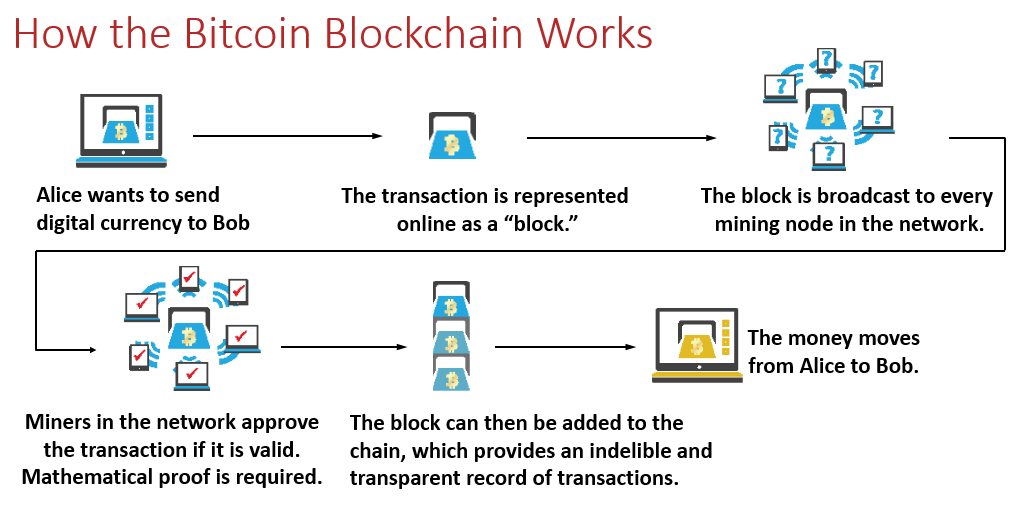
\includegraphics[width=1.0\textwidth]{./images/BitcoinTransaction.png}
      \caption[How the Bitcoin blockchain propagates transactions]{How the Bitcoin blockchain propagates transactions \protect\footnotemark}
       \label{fig:bitcoin-transaction}
\end{figure}
\footnotetext{Image source: D.Sleeter, "The Promise of Blockchain Technology," Jan. 2017. [Online]}

An example transaction is shown in Figure \ref{fig:bitcoin-transaction} above. If a user \textit{Alice} wishes to send another user \textit{Bob} digital currency from her wallet, she needs to first obtain the public address of Bob's wallet to create a new transaction. This transaction contains Bob's address, the payment amount, and the network fee. Alice must then sign this transaction with her private key, which proves to the network that she has cryptographic ownership of her corresponding wallet address. Alice then broadcasts this transaction on the blockchain, where it is received by other machines known as \textit{miners}.

\subsection{Distributed Consensus}
Bitcoin replaces a centralised payment ledger with a distributed one, but the problem arises of ensuring these transactions are ordered in a synchronised way. In the transaction between Alice and Bob above, the network needs to ensure that the coins being sent exist in Alice's wallet, and cannot be sent twice. This is referred to as the \textit{double spending} problem \cite{hoepman_distributed_2007}. 

A \textit{proof-of-work} verification system is used to tackle this. It specifies a certain algorithm which takes a non-trivial amount of processing power time to compute but conversely the solution is trivial to validate. 

When a transaction is broadcast to the network and received by a node, it is bundled with other unconfirmed transactions into a \textit{transaction block}. This block contains a list of transactions, a link to the previous block, and a random nonce number. This number is incremented until the computed hash of the block including this nonce begins with a specified number of zeros, thus providing a method of proof of work.

Calculating this hash correctly is computationally intensive, and ensures that a certain amount of computing power is required to validate a block. Once a block has been created with the desired hash, as shown in the figure above, it is broadcast to the network, and other nodes can verify its legitimacy by adding it to the end of their chain of blocks. This block is now considered \textit{valid}, and the order of transactions within the chain is thus preserved. 

In return for using computing power to verify blocks, the operator of the mining node receives some freshly generated Bitcoin currency in their wallet, as well as the network fees that users included in their transactions. This block reward began at \textit{50 BTC}, but it has been halved twice since to combat inflation and now stands at \textit{12.5 BTC} per block mined at the time of writing.

A key strength that comes with the ordering of transactions is that each transaction can be traced back to the original block where its source Bitcoin was minted. Before a Bitcoin node can start to mine and verify blocks of transactions, it must first download the entire history of transactions since the blockchain inception and verify each one independently. Only then does it begin to verify new transactions and add them to the blockchain.

\section{Ethereum}
Ethereum was released as an \textit{"alternative protocol for building decentralised applications"} \cite{buterin_ethereum:_2014}. It builds on the blockchain features described in Bitcoin above, by adding programmability and scalability to the network. Ethereum does not just represent a digital currency, as Bitcoin does, but also allows many other use cases to be stored as application-level code on the blockchain.

\subsection{Smart Contracts}
Ethereum contains smart contracts, which are computer programs compiled and stored in the Ethereum blockchain. These are assigned addresses and can receive currency transactions just like standard wallets, but their functions can also be initiated with special types of function call transactions.

Smart contracts can accept parameters, store state, manipulate internal state as a result of function calls, and return data in responses. This added functionality is not present in the Bitcoin blockchain, and it comes with distinct advantages. Application logic is performed and displayed transparently on the public blockchain, the internal state is available openly for scrutinising, and the operations are completely autonomous. They provide cryptographically auditable, append-only ledgers for building a new era of decentralised applications.

\subsection{Ethereum Virtual Machine}
Ethereum miner nodes are required to verify all state changes as blocks are propagated through the network. Application level code that is executed within smart contracts is considered a state change that is performed by the network via consensus. 

To achieve this consensus through code execution, the \textit{Ethereum Virtual Machine} was developed. This allows mining nodes to run code of arbitrary algorithmic complexity in a deterministic manner, and to reach consensus on the outcome of the computation. Smart contract operation is parallelised across all nodes in the network, which ensures fault tolerance, zero downtime, and permanent irrefutable state changes.

In the same way that Bitcoin miners accept network fees for verifying transactions, Ethereum miners that compute smart contracts receive fees for program execution. This is called the \textit{gas price} of the transaction. The sender must pay for each line of code the program executes, including computation, events and storage. This is to discourage attacks like infinite loops in code from affecting the network.

\subsection{Discussion}
Ethereum provides secure transfers of value, auditable and autonomous program execution, fault-tolerant redundant storage, and an immutable record of information. This makes it a powerful platform on which to tackle global problems in a new decentralised paradigm. It's been considered as the first \textit{Global Computer}, capable of operating completely censorship-free and across international borders.

The Ethereum platform has been chosen for the system design in this paper as it addresses many of the problems with centralised identity management. This is further outlined in the Solution Overview and Implementation details in Chapters \ref{chp:solution-design} and \ref{chp:implementation}.

\section{Decentralised Storage}
After the introduction of the blockchain, decentralised storage solutions have arisen that offer redundant hosting of long-form information and files. They present the following advantages:
\begin{itemize}
	\item Low-latency data retrieval
    \item Efficient content caching
    \item Reliable fault-tolerant storage
    \item Censorship resistance
    \item File versioning and archival functionality
\end{itemize}
Some notable implementations are discussed below.

\subsection{IPFS}
\ac{IPFS} \cite{benet_ipfs_2014} is a content-addressed distributed file system supported by a peer-to-peer network of machines. It can operate on any transport protocol and uses \acp{DHT} for peer identification and routeing. It provides cryptographic-hash content addressing, file integrity, and filesystem encryption and signing.

\ac{IPFS} also supports a name service known as the \ac{IPNS} for the persistent naming of dynamic content. This allows for routeing of a static name to the hash of a file and is based on access control concepts from \ac{PKI}.

The function of \ac{IPFS} is similar to Bittorrent, whereby nodes serve local copies of content to the network. When files are requested, the local node caches the response and continues to seed the file back to the network. If all nodes serving a file go offline, then the file is no longer available. An economic incentive such as Filecoin \cite{filecoin.io_filecoin:_2014} has been suggested as an addition to the protocol, which would encourage nodes to continue serving content for financial reward.

\subsection{Swarm}
Swarm \cite{noauthor_swarm_nodate} is a distributed storage platform and content distribution network similar to \ac{IPFS}. Both projects provide decentralised storage of content-addressed files split into chunks.

Swarm is distinct in that it runs on the Ethereum peer-to-peer networking layer, and was developed in the context of close integration with the Ethereum blockchain. It also supports incentivised system benefits through smart contracts native to Ethereum via the pool of network peers.

Swarm is slightly behind \ac{IPFS} in terms of development and global reach, and it is possible that the two projects could integrate together sometime in the future \cite{ethersphere_ipfs_2017}.

\subsection{Discussion}
Decentralised storage is cheaper than using Ethereum contract storage, and it does not bloat the network with large amounts of data. It is therefore seen as valuable to use an external decentralised storage system for the solution proposed in this paper.

\section{Blockchain Identity Systems}
\label{sec:blockchain-identity}
\subsection{Blockstack}
Blockstack \cite{blockstack_inc._blockstack:_2017} is a decentralised identity, discovery and storage platform, built on blockchain technology. It makes use of virtualchains \cite{j_nelson_extending_2016} that allow the output of arbitrary state machines to be pinned to underlying blockchain infrastructure. 

Blockstack is similar to Ethereum in that it supports decentralised applications, but instead performs its computation off-chain. The underlying blockchain technology is used to authenticate an application before it is run by the user. Applications are not Turing-complete by design, but they can interface with the Turing-complete Ethereum blockchain by use of a virtualchain.

Blockstack supports an identity project known as Onename, which allows users to register an identity on the Blockstack network. This features peer-to-peer identity attestations and verifications. Originally Onename used the Namecoin blockchain as its infrastructure, but changed to Bitcoin instead in response to centralised-mining and spam issues with Namecoin \cite{kyle_torpey_3_2015}. 

Although Onename supports a decentralised blockchain-based identity service, it still relies on off-chain computation using Blockstack with many layers of resolvers and verifiers \cite{onename_introducing_2015}. The lack of a stable and transparent network supporting the system reduces the usefulness of the project.

\subsection{Estonian e-Residency}
The Republic of Estonia released a state digital identity system known as e-Residency in 2014 \cite{the_digital_society_estonian_2014}. It is a transnational secure identity offered by the government and supported by a physical smart card.

Citizens apply to the government with their legal information, including copies of their fingerprints, before being issued a digital identity. Residents can use the system for company registration, banking, payment services and document signing. 

The cards use 2048-bit RSA encryption for document signing and verification. Legal documents can be digitally signed using this technology, with the full support of the Estonian legal system. The system currently does not use blockchain-based infrastructure, but it has partnered with initiatives like Identit.ee \cite{noauthor_identit.ee_nodate} and Bitnation \cite{bitnation_estonia_2015} to pursue this in the future.

\subsection{Evernym}
Evernym \cite{smith_identity_2016} is an identity system built on the permissioned \ac{DLT} known as Sovrin, which is dedicated solely to decentralised identity.

The Sovrin network is supported by the Sovrin Foundation, and it consists of interconnected nodes forming a consensus on a shared ledger. Users create self-sovereign identities with personal attributes, and request claims from trusted third parties to build reputation.

Currently, there is no financial incentive to host a Sovrin node, so the majority of the network is research-focused. The network plans to introduce premium claims in the future to provide rewards to nodes that distribute and verify identities \cite{sovrin_foundation_sovrin_nodate}. 

\subsection{ShoCard}
ShoCard \cite{shocard_inc._shocard:_2016} is a digital identity application focusing on user identification in the travel sector. It offers a mobile application for storing identities, while also pinning hashed and signed identity data to the Bitcoin blockchain.

Users scan their document with the application, which reads each \ac{MRZ} and stores an encrypted version on the device. Each field is then one-way hashed, signed with the user's private key, and published to the blockchain.

Disclosure of user data is done by encrypting the local copy of information with the receiver's public key and transferring it via a QR code. The receiver can then validate the information against the signed version published on the blockchain. 

ShoCard specifies that the receiving party, such as an airline gate agent, checks the digital copy against the physical passport before proceeding. The airline can then create certification records confirming this physical and digital link, and hand them back to the user. This is referred to as a \textit{travel token}. The user can then present this token at subsequent passenger checks to streamline verification. However, each checkpoint is still required to compare the token against the blockchain. This is done to check for continued validity and possible revocation of the token.

ShoCard presents a useful data disclosure process, ensuring transferred data is checked against the blockchain during each transaction. It fails to support any key or identity recovery protocols, however, and is inherently tied to identity supported by physical documents only.

\subsection{uPort}
\label{sec:uport}
uPort is a self-sovereign identity platform built on the Ethereum blockchain. At its core, it utilises a network of smart contracts for each user and offers a mobile application and accompanying developer libraries.

The uPort mobile application generates a public and private key for a user and deploys smart contracts to represent their identity. It deploys what is known as the \textit{Proxy Contract} to represent the user's unique identifier, the \textit{Controller Contract} to provide identity access control logic, and the \textit{Recovery Quorum Contract} to facilitate the recovery of the user's identity. It also stores pointers to these contracts in a centralised \textit{Registry Contract}.

uPort presents a novel recovery concept for digital identity, where a quorum of the user's friends can collaborate to restore access to an identity. Friends can vote to replace the ownership key of an identity with a newly-generated one, and the identity contract logic performs this request when a majority consensus is reached.

uPort retains some centralised elements, as it uses a centralised messaging server to transfer attribute information from a user's device, a push notification system and application manager. It also requires the use of a central registry to log the mapping of user public keys to unique identifiers for convenience. These elements are deemed necessary by the project for initial user onboarding, but have the potential to be removed in the future \cite{braendgaard_response:_2017}.

In addition, uPort does not support the recovery of private data, as this is stored off-chain on the user's device. Sensitive data cannot be stored in public form on the blockchain without first being encrypted. This research identifies a possible approach to allow this data to be recovered.

\subsection{Discussion}
There are many approaches to providing self-sovereign in the digital space, with promising blockchain implementations. The primary areas of interest that remain unsolved are completely decentralised systems that support the recovery of private identity data. 

The focus of this research is to propose a solution that builds upon the advancements of existing work in the field, and to use stable and transparent blockchain architecture with complete privacy and adequate recoverability.